\documentclass[11pt,a4paper]{article}

\usepackage[utf8]{inputenc}
\usepackage[T1]{fontenc}
\usepackage{lmodern}
\usepackage{float}
\usepackage[margin=2cm]{geometry}
\usepackage{amsmath,amssymb}
\usepackage{booktabs}
\usepackage{graphicx}
\usepackage{hyperref}
\usepackage{xcolor}
\usepackage{titlesec}
\usepackage{tabularx}

\hypersetup{
    colorlinks=true,
    linkcolor=blue!70!black,
    citecolor=blue!70!black,
    urlcolor=blue!70!black
}

\titleformat{\section}{\large\bfseries}{\thesection.}{0.5em}{}
\titleformat{\subsection}{\normalsize\bfseries}{\thesubsection.}{0.5em}{}
\titlespacing*{\section}{0pt}{1.2ex plus 0.5ex minus .2ex}{0.6ex}
\titlespacing*{\subsection}{0pt}{1.0ex plus 0.4ex minus .2ex}{0.4ex}
\setlength{\parskip}{0.45em}
\setlength{\parindent}{0pt}

% ----------------------------------------------------------------------
% Resultados numéricos (preenchidos a partir dos CSVs gerados em results/).
% ----------------------------------------------------------------------
\newcommand{\WINDOW}{24}
\newcommand{\HORIZON}{6}
\newcommand{\GAP}{30}
\newcommand{\RAINTH}{0,2}
\newcommand{\NREG}{26304}
\newcommand{\NFEAT}{13}
\newcommand{\NWIN}{26275}
\newcommand{\POSRATE}{0,1721}
\newcommand{\SPLITRATES}{%
Cronol\'ogica & Treino & 18362 & 0,1784 \\
Cronol\'ogica & Valida\c c\~ao & 3881 & 0,1301 \\
Cronol\'ogica & Teste & 3912 & 0,1897 \\
Aleat\'oria & Treino & 18392 & 0,1723 \\
Aleat\'oria & Valida\c c\~ao & 3941 & 0,1675 \\
Aleat\'oria & Teste & 3942 & 0,1761 \\
}
\newcommand{\BESTCONFIGS}{%
Cronol\'ogica & GRU & 64 & 2 & 0,7002 & 0,4747 \\
Aleat\'oria & LSTM & 64 & 2 & 0,2281 & 0,8709 \\
}
\newcommand{\TESTRESULTS}{%
Cronol\'ogica & GRU & 0,7717 & 0,4473 & 0,8639 & 0,5894 & 0,8960 \\
Aleat\'oria & LSTM & 0,9444 & 0,7851 & 0,9424 & 0,8566 & 0,9844 \\
}
\newcommand{\SPLITCOMPARISON}{%
Acur\'acia & 0,7717 & 0,9444 & 0,1727 \\
Precis\~ao & 0,4473 & 0,7851 & 0,3378 \\
Revoca\c c\~ao & 0,8639 & 0,9424 & 0,0785 \\
F1 & 0,5894 & 0,8566 & 0,2672 \\
AUC & 0,8960 & 0,9844 & 0,0884 \\
}


\begin{document}

\begin{center}
{\LARGE \textbf{Projeto 4: Classificação de Chuva em Série Temporal com
Redes Recorrentes (LSTM e GRU)}} \\[0.35em]
{\large Disciplina: Introdução às Redes Neurais Artificiais} \\[0.3em]
\textbf{Autora:} Gabriely Di Folco Rocha (RA: 188892) \\[0.2em]
\textbf{Repositório:} \url{https://github.com/ghostfoxgoddes3/ANN}
\end{center}

\vspace{-0.5em}
\hrule
\vspace{0.8em}

\section{Introdução e Motivação Ecológico-Social}

Este projeto trata da classificação de séries temporais meteorológicas: dada
uma janela de observações horárias recentes, o modelo prevê se haverá chuva
nas próximas horas. A tarefa é formulada como classificação binária -- ``vai
chover'' versus ``não vai chover'' em um horizonte de \HORIZON{} horas.

A escolha do problema não é neutra. Os anos cobertos pelos dados
(2022--2024) incluem o episódio de \textbf{El Ni{\~n}o} forte de 2023--2024, um
dos mais intensos já registrados. O El Ni{\~n}o Oscila{\c c}{\~a}o Sul (ENOS)
é um fen{\^o}meno acoplado oceano--atmosfera no Pac{\'i}fico Equatorial que
altera a circula{\c c}{\~a}o atmosf{\'e}rica e o transporte de umidade,
afetando a precipita{\c c}{\~a}o em todo o Brasil~\cite{noaa_oni,
enso_subtropical2026}. Estudos de atribui{\c c}{\~a}o indicam que as mudan{\c
c}as clim{\'a}ticas, combinadas ao El Ni{\~n}o, dobraram a probabilidade de
eventos extremos como as chuvas que atingiram o Rio Grande do Sul em maio de
2024~\cite{rodrigues2024rs}.

Esse contexto motiva duas decis{\~o}es do projeto. Primeiro, incorporamos o
{\'i}ndice ONI (\textit{Oceanic Ni{\~n}o Index}) como vari{\'a}vel ex{\'o}gena,
permitindo que o modelo tenha acesso ao estado de larga escala do clima.
Segundo, a discuss{\~a}o dos resultados considera que a crescente frequ{\^e}ncia
de eventos extremos torna a previs{\~a}o de curto prazo socialmente relevante:
sistemas de alerta dependem de modelos que generalizem para o futuro, e n{\~a}o
apenas para o passado j{\'a} observado.

\section{Configuração Experimental e Reprodutibilidade}

\subsection{Fonte e Caracterização dos Dados}

Os dados meteorol{\'o}gicos s{\~a}o da esta{\c c}{\~a}o autom{\'a}tica
\texttt{A701} (S{\~a}o Paulo -- Mirante) do INMET~\cite{inmet}, com
resolu{\c c}{\~a}o hor{\'a}ria. Foram utilizados os anos de 2022 a 2024,
totalizando \NREG{} registros hor{\'a}rios ap{\'o}s a padroniza{\c c}{\~a}o
do formato (codifica{\c c}{\~a}o \textit{latin1}, separador \texttt{;},
decimal com v{\'i}rgula e oito linhas de metadados).

Cada instante {\'e} descrito por vari{\'a}veis de superf{\'i}cie:
precipita{\c c}{\~a}o, press{\~a}o, radia{\c c}{\~a}o global, temperatura do
ar, temperatura do ponto de orvalho, umidade relativa, dire{\c c}{\~a}o e
velocidade do vento. A essas vari{\'a}veis acrescentamos quatro atributos
c{\'i}clicos -- seno e cosseno da hora do dia e do dia do ano -- e o
{\'i}ndice ONI mensal, totalizando \NFEAT{} vari{\'a}veis de entrada.

Lacunas curtas foram interpoladas (limite de seis horas) e a
precipita{\c c}{\~a}o ausente foi tratada como zero. A grade temporal foi
regularizada para passo hor{\'a}rio cont{\'i}nuo.

\subsection{Construção das Janelas e do Rótulo}

A entrada da rede {\'e} uma janela deslizante de \WINDOW{} horas. O
r{\'o}tulo associado ao instante $t$ (final da janela) {\'e}

\[
y_t =
\begin{cases}
1, & \text{se } \sum_{k=1}^{\HORIZON} \text{precip}_{t+k} \ge
\RAINTH\ \text{mm} \\[0.4em]
0, & \text{caso contr{\'a}rio.}
\end{cases}
\]

Ou seja, a classe positiva indica chuva acumulada acima de \RAINTH\ mm nas
pr{\'o}ximas \HORIZON{} horas. O deslizamento da janela gerou \NWIN{} exemplos,
dos quais \POSRATE\ pertencem {\`a} classe positiva. Esse desbalanceamento
($\approx$ 1 chuva para cada 5 janelas) {\'e} realista e exige m{\'e}tricas
al{\'e}m da acur{\'a}cia.

\subsection{As Duas Estratégias de Partição}

O ponto conceitual central do projeto {\'e} a compara{\c c}{\~a}o entre duas
formas de dividir os dados, ambas com propor{\c c}{\~a}o 70/15/15 para
treino/valida{\c c}{\~a}o/teste.

\textbf{Parti{\c c}{\~a}o cronol{\'o}gica (principal).} Blocos cont{\'i}guos
no tempo: o modelo treina no passado, ajusta hiperpar{\^a}metros no per{\'i}odo
intermedi{\'a}rio e {\'e} testado no futuro. Entre os blocos aplicamos um
\textit{embargo} (\textit{gap}) de \GAP{} janelas, descartando as janelas de
fronteira que se sobreporiam. Essa {\'e} a avalia{\c c}{\~a}o honesta, pois
reproduz o uso real do modelo.

\textbf{Parti{\c c}{\~a}o aleat{\'o}ria (did{\'a}tica).} As janelas s{\~a}o
embaralhadas e sorteadas. Como janelas vizinhas compartilham instantes, uma
janela de valida{\c c}{\~a}o ou teste quase sempre se sobrep{\~o}e a uma de
treino -- fen{\^o}meno conhecido como \textit{vazamento temporal}
(\textit{temporal leakage}). A m{\'e}trica resultante tende a ser otimista e
n{\~a}o reflete o desempenho em dados realmente novos~\cite{bergmeir2012cv}.

Mantemos as duas parti{\c c}{\~o}es justamente para \emph{medir} o quanto o
vazamento infla o desempenho aparente. A Tabela~\ref{tab:split_rates} mostra
ainda que a taxa da classe positiva varia entre os blocos cronol{\'o}gicos,
enquanto permanece praticamente constante na parti{\c c}{\~a}o aleat{\'o}ria,
evid{\^e}ncia direta da n{\~a}o estacionariedade da s{\'e}rie.

\begin{table}[H]
\centering
\small
\caption{Tamanho dos conjuntos e taxa da classe ``chuva'' por parti{\c
c}{\~a}o.}
\label{tab:split_rates}
\begin{tabular}{llrr}
\toprule
\textbf{Parti{\c c}{\~a}o} & \textbf{Conjunto} & \textbf{Janelas} &
\textbf{Taxa de chuva} \\
\midrule
\SPLITRATES
\bottomrule
\end{tabular}
\end{table}

\subsection{Modelo, Treino e Reprodutibilidade}

O modelo {\'e} uma rede recorrente (LSTM~\cite{hochreiter1997lstm} ou
GRU~\cite{cho2014gru}, selecion{\'a}vel) que processa a janela e usa o estado
oculto do {\'u}ltimo instante em uma cabe{\c c}a linear, produzindo o
\textit{logit} da classe ``chuva''. O treino usa
\texttt{BCEWithLogitsLoss} com \texttt{pos\_weight} igual {\`a} raz{\~a}o
negativos/positivos, compensando o desbalanceamento.

A padroniza{\c c}{\~a}o das vari{\'a}veis foi ajustada \textbf{somente no
conjunto de treino} e aplicada aos demais, evitando vazamento de escala. A
otimiza{\c c}{\~a}o usou Adam, com \textit{early stopping} monitorando a loss
de valida{\c c}{\~a}o (\textit{patience} de 10 {\'e}pocas, m{\'a}ximo de 100).
A semente foi fixada em 42.

\section{Ajuste de Hiperparâmetros}

A busca percorreu um \textit{grid} variando a c{\'e}lula (LSTM/GRU), o tamanho
do estado oculto (32 e 64) e o n{\'u}mero de camadas (1 e 2), com taxa de
aprendizado $10^{-3}$ e \textit{batch} 128. O crit{\'e}rio foi a menor loss de
valida{\c c}{\~a}o, com o teste mantido intocado. A busca foi conduzida
separadamente para cada parti{\c c}{\~a}o.

\begin{table}[H]
\centering
\small
\caption{Melhor configura{\c c}{\~a}o por parti{\c c}{\~a}o (sele{\c c}{\~a}o
pela loss de valida{\c c}{\~a}o).}
\label{tab:best_configs}
\begin{tabular}{llrrrr}
\toprule
\textbf{Parti{\c c}{\~a}o} & \textbf{C{\'e}lula} & \textbf{Oculto} &
\textbf{Camadas} & \textbf{Loss val.} & \textbf{F1 val.} \\
\midrule
\BESTCONFIGS
\bottomrule
\end{tabular}
\end{table}

\section{Dinâmica de Treinamento}

As curvas de loss e F1 (Figuras~\ref{fig:curves_chrono}
e~\ref{fig:curves_random}) mostram a converg{\^e}ncia dos modelos finais. O
\textit{early stopping} seleciona o estado de menor loss de valida{\c c}{\~a}o.

\begin{figure}[H]
\centering
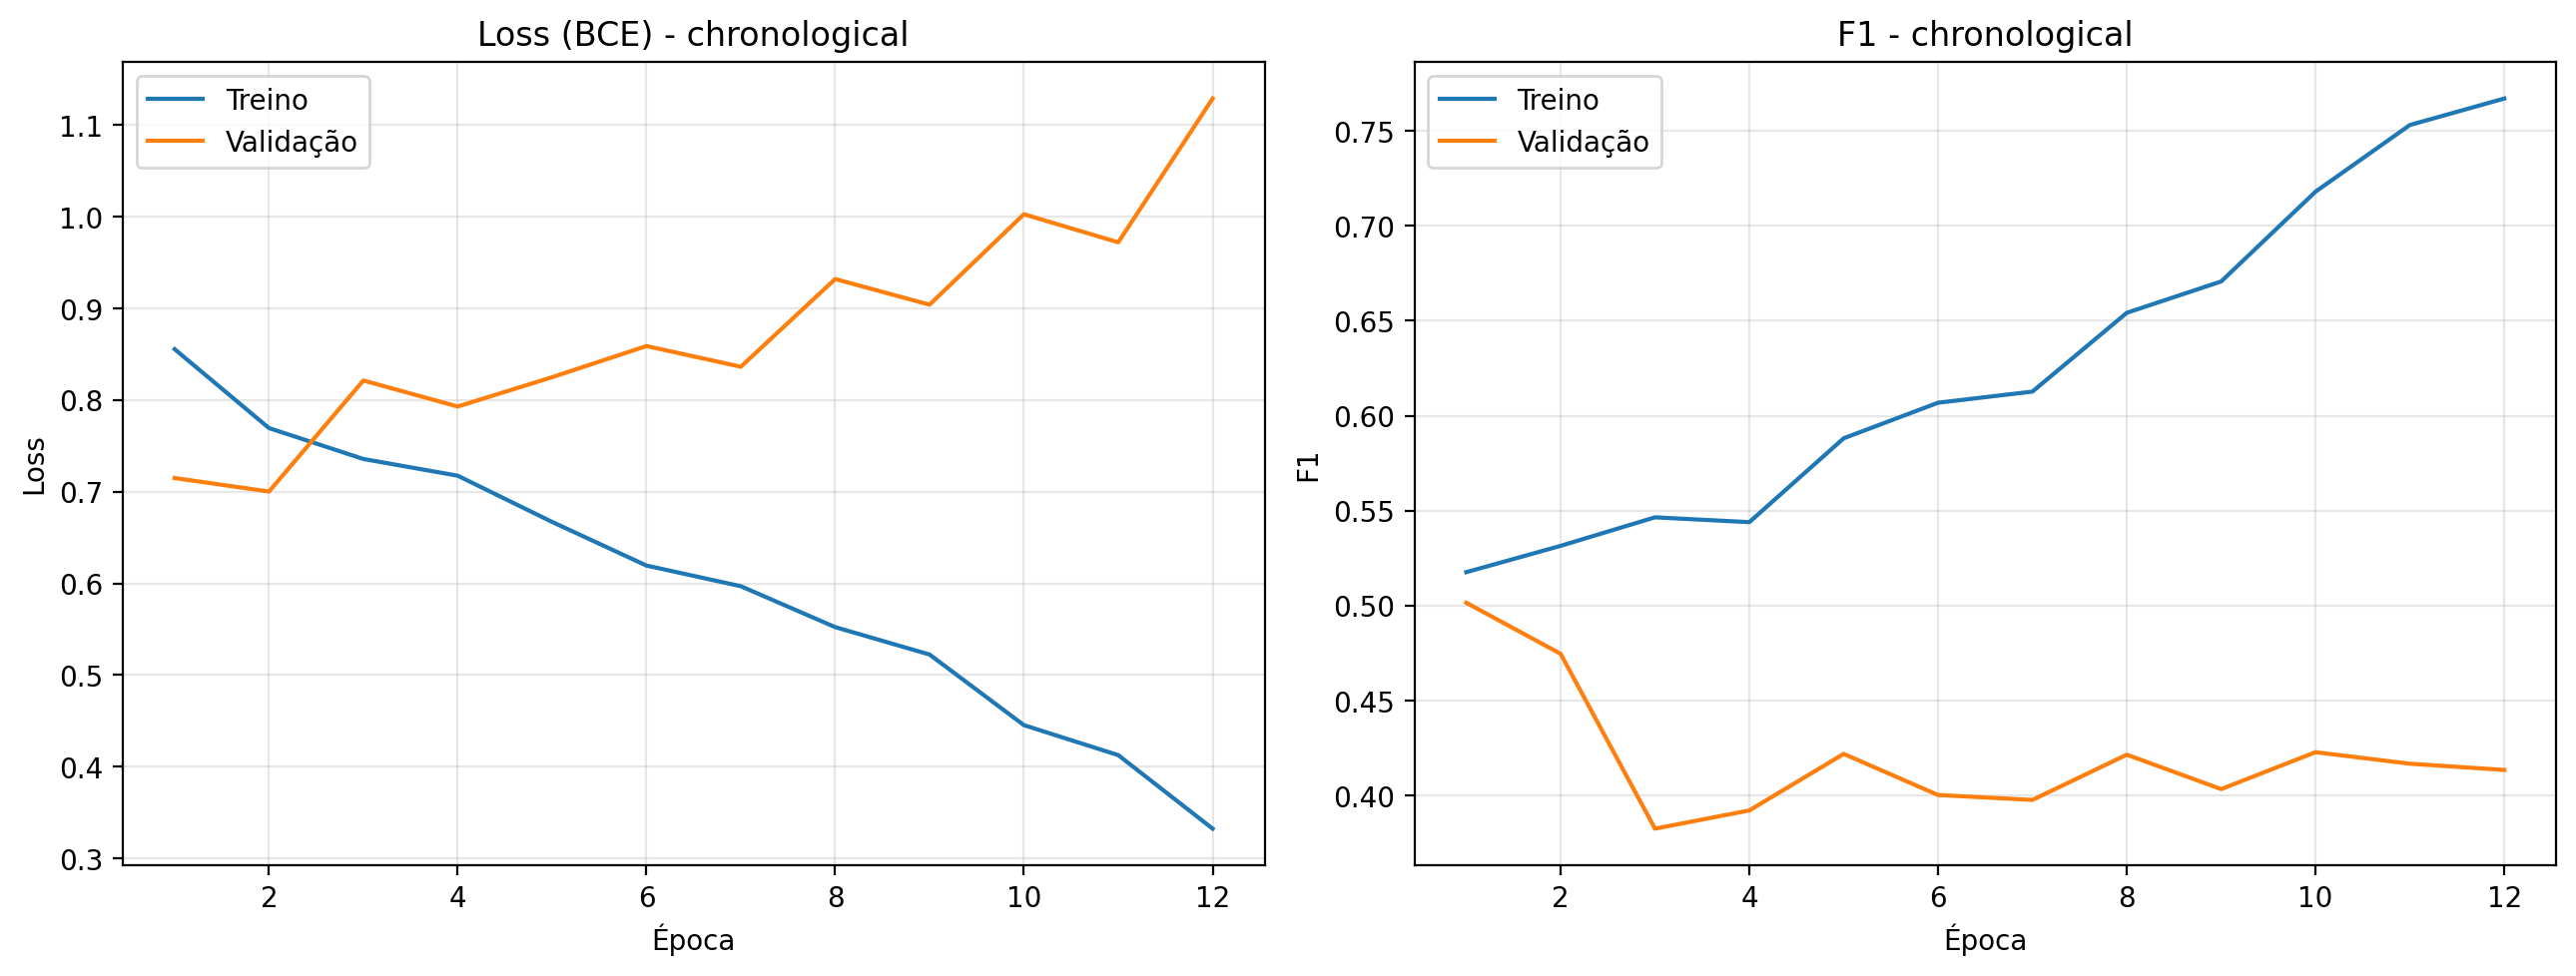
\includegraphics[width=\textwidth]{../figures/curves_chronological.png}
\caption{Curvas de aprendizagem (loss e F1) na parti{\c c}{\~a}o
cronol{\'o}gica.}
\label{fig:curves_chrono}
\end{figure}

\begin{figure}[H]
\centering
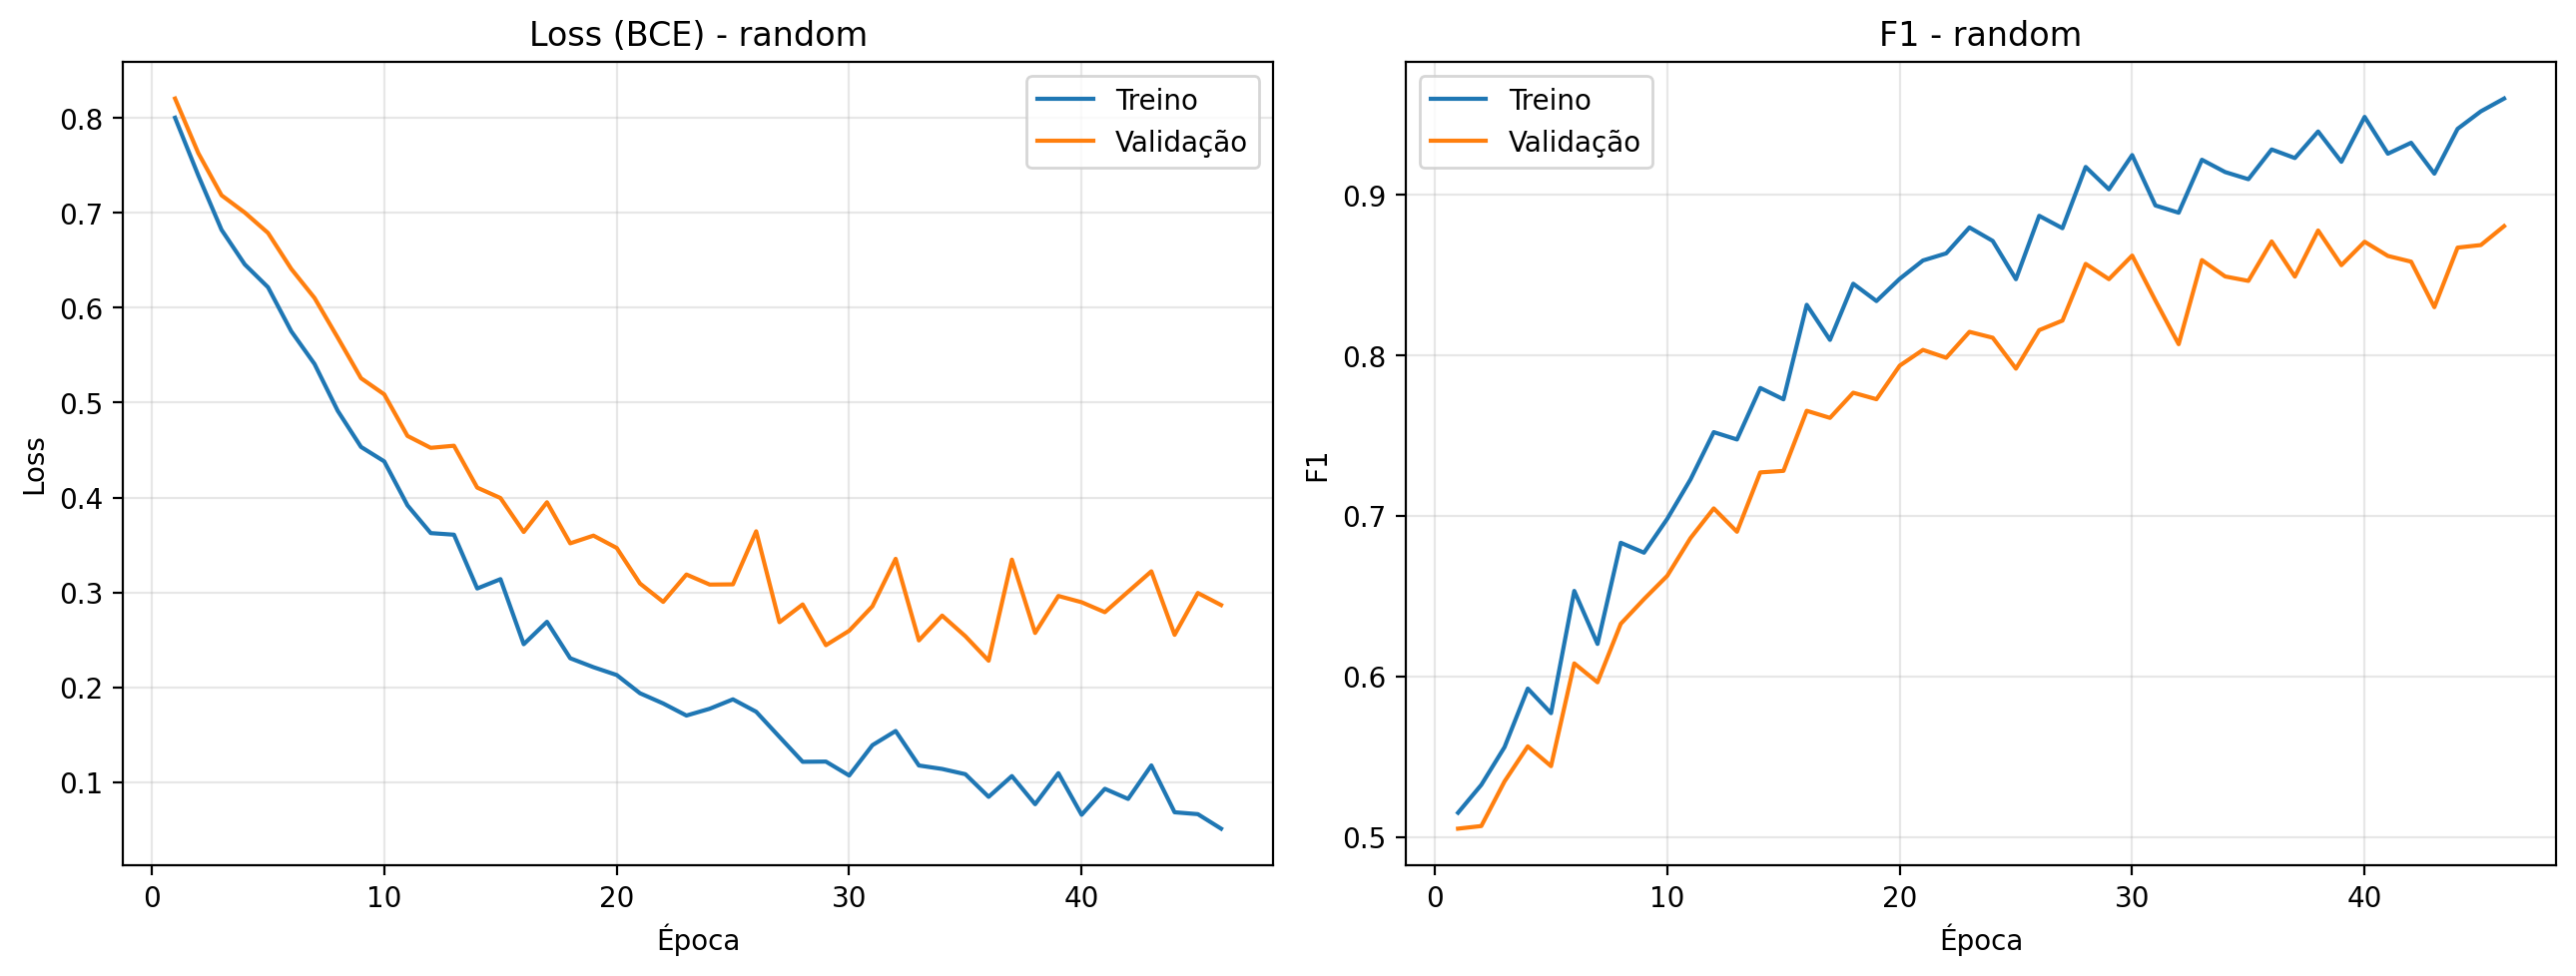
\includegraphics[width=\textwidth]{../figures/curves_random.png}
\caption{Curvas de aprendizagem (loss e F1) na parti{\c c}{\~a}o
aleat{\'o}ria.}
\label{fig:curves_random}
\end{figure}

\section{Avaliação no Teste e o Efeito do Vazamento Temporal}

A Tabela~\ref{tab:test} apresenta o desempenho no conjunto de teste de cada
parti{\c c}{\~a}o. A compara{\c c}{\~a}o deve ser lida com aten{\c c}{\~a}o: a
parti{\c c}{\~a}o aleat{\'o}ria \emph{n{\~a}o} corresponde a uma avalia{\c
c}{\~a}o v{\'a}lida, e sua presen{\c c}a serve para quantificar o vi{\'e}s
introduzido pelo vazamento.

\begin{table}[H]
\centering
\small
\caption{Desempenho no conjunto de teste por parti{\c c}{\~a}o.}
\label{tab:test}
\begin{tabular}{llrrrrr}
\toprule
\textbf{Parti{\c c}{\~a}o} & \textbf{C{\'e}lula} & \textbf{Acur.} &
\textbf{Prec.} & \textbf{Rev.} & \textbf{F1} & \textbf{AUC} \\
\midrule
\TESTRESULTS
\bottomrule
\end{tabular}
\end{table}

\begin{table}[H]
\centering
\small
\caption{Diferen{\c c}a entre as parti{\c c}{\~o}es (aleat{\'o}ria menos
cronol{\'o}gica). Valores positivos indicam desempenho artificialmente mais
alto sob vazamento.}
\label{tab:split_comparison}
\begin{tabular}{lrrr}
\toprule
\textbf{M{\'e}trica} & \textbf{Cronol{\'o}gico} & \textbf{Aleat{\'o}rio} &
\textbf{Dif.} \\
\midrule
\SPLITCOMPARISON
\bottomrule
\end{tabular}
\end{table}

\begin{figure}[H]
\centering
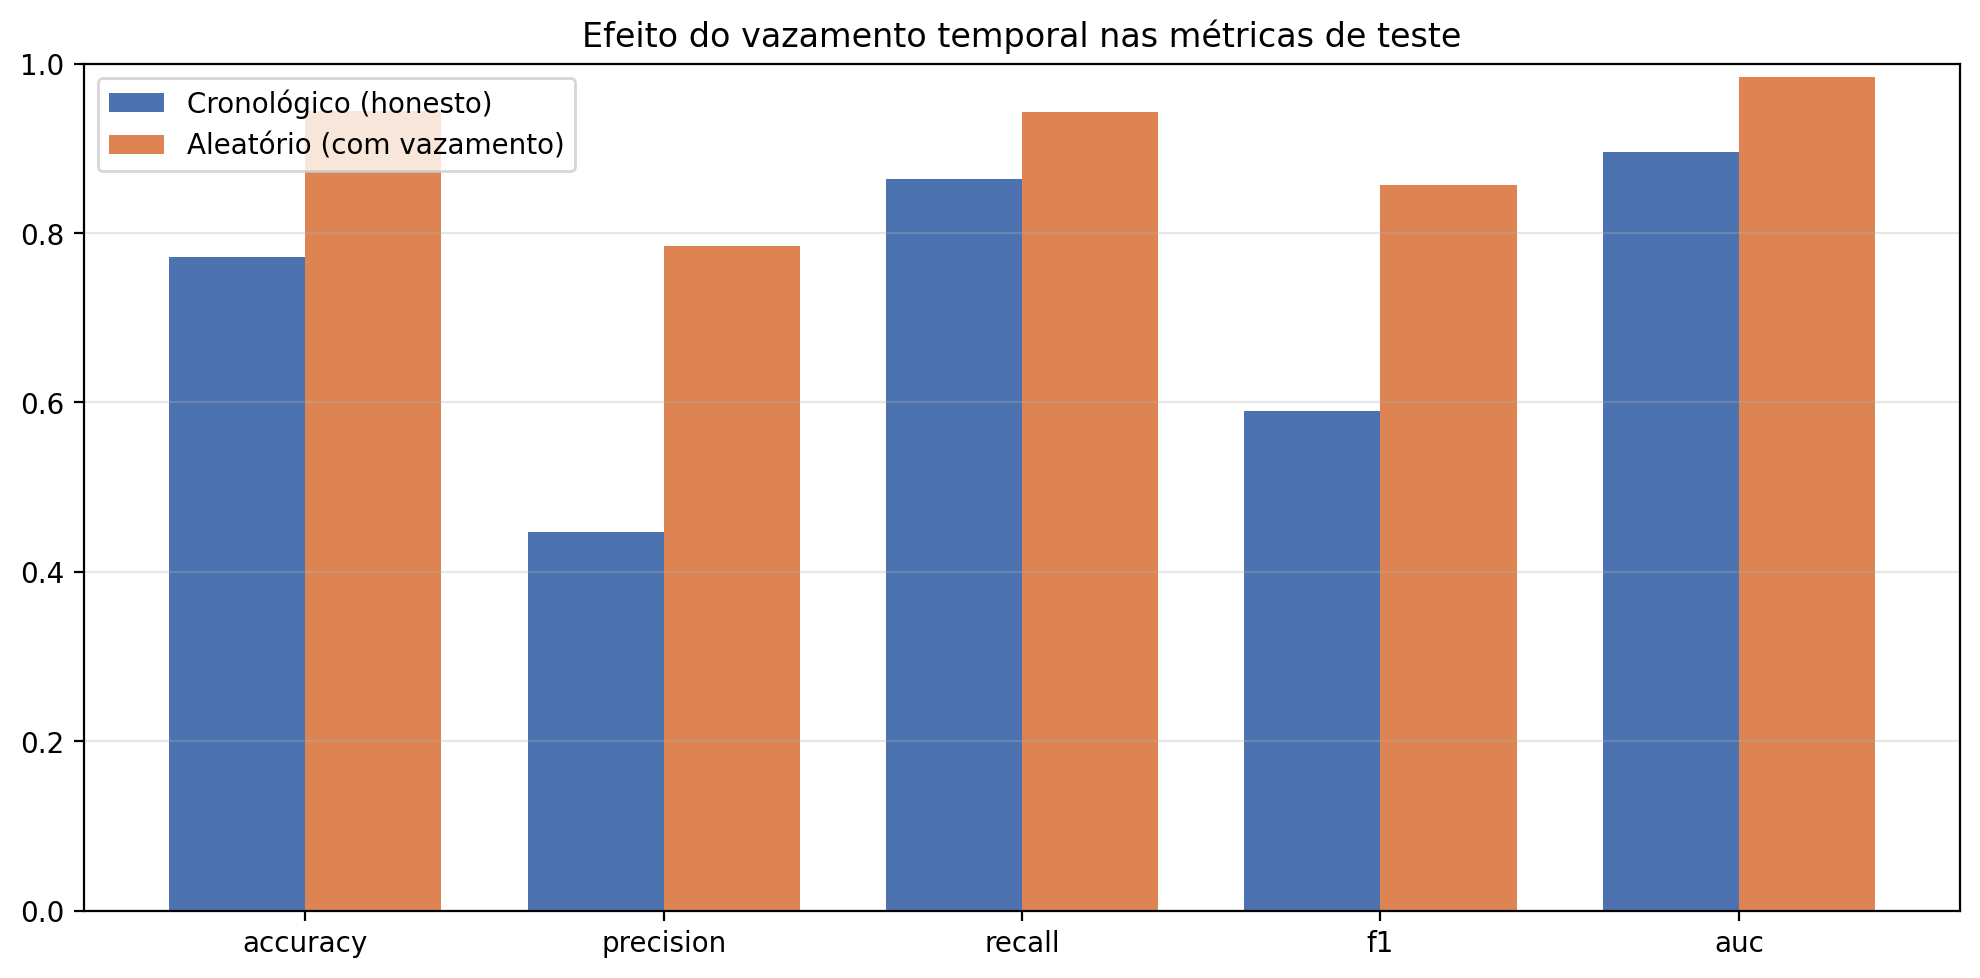
\includegraphics[width=0.85\textwidth]{../figures/split_metric_comparison.png}
\caption{Compara{\c c}{\~a}o visual das m{\'e}tricas de teste entre as duas
parti{\c c}{\~o}es.}
\label{fig:split_comparison}
\end{figure}

\begin{figure}[H]
\centering
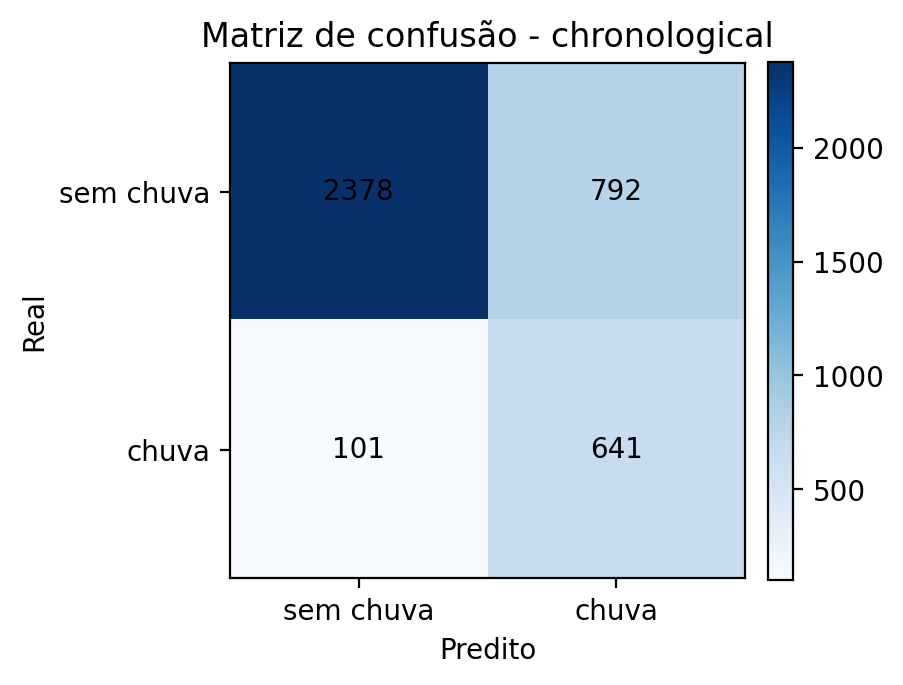
\includegraphics[width=0.48\textwidth]{../figures/confusion_chronological.png}
\hfill
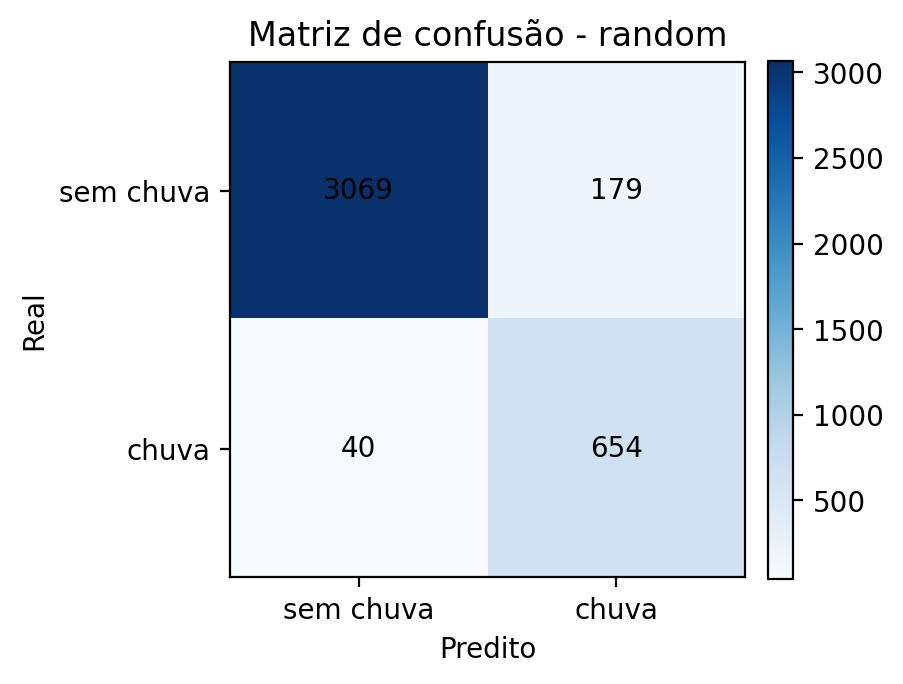
\includegraphics[width=0.48\textwidth]{../figures/confusion_random.png}
\caption{Matrizes de confus{\~a}o: cronol{\'o}gica (esquerda) e aleat{\'o}ria
(direita).}
\label{fig:confusion}
\end{figure}

\section{Contexto Climático e Discussão Ecológico-Social}

A Figura~\ref{fig:climate} sobrep{\~o}e o {\'i}ndice ONI {\`a}
precipita{\c c}{\~a}o mensal da esta{\c c}{\~a}o. Valores de ONI acima de
$0{,}5\,^{\circ}$C caracterizam El Ni{\~n}o; o per{\'i}odo 2023--2024 aparece
como um epis{\'o}dio forte. A Figura~\ref{fig:nonstat} mostra a taxa mensal da
classe ``chuva'', cuja varia{\c c}{\~a}o ao longo do tempo evidencia a
n{\~a}o estacionariedade da s{\'e}rie.

\begin{figure}[H]
\centering
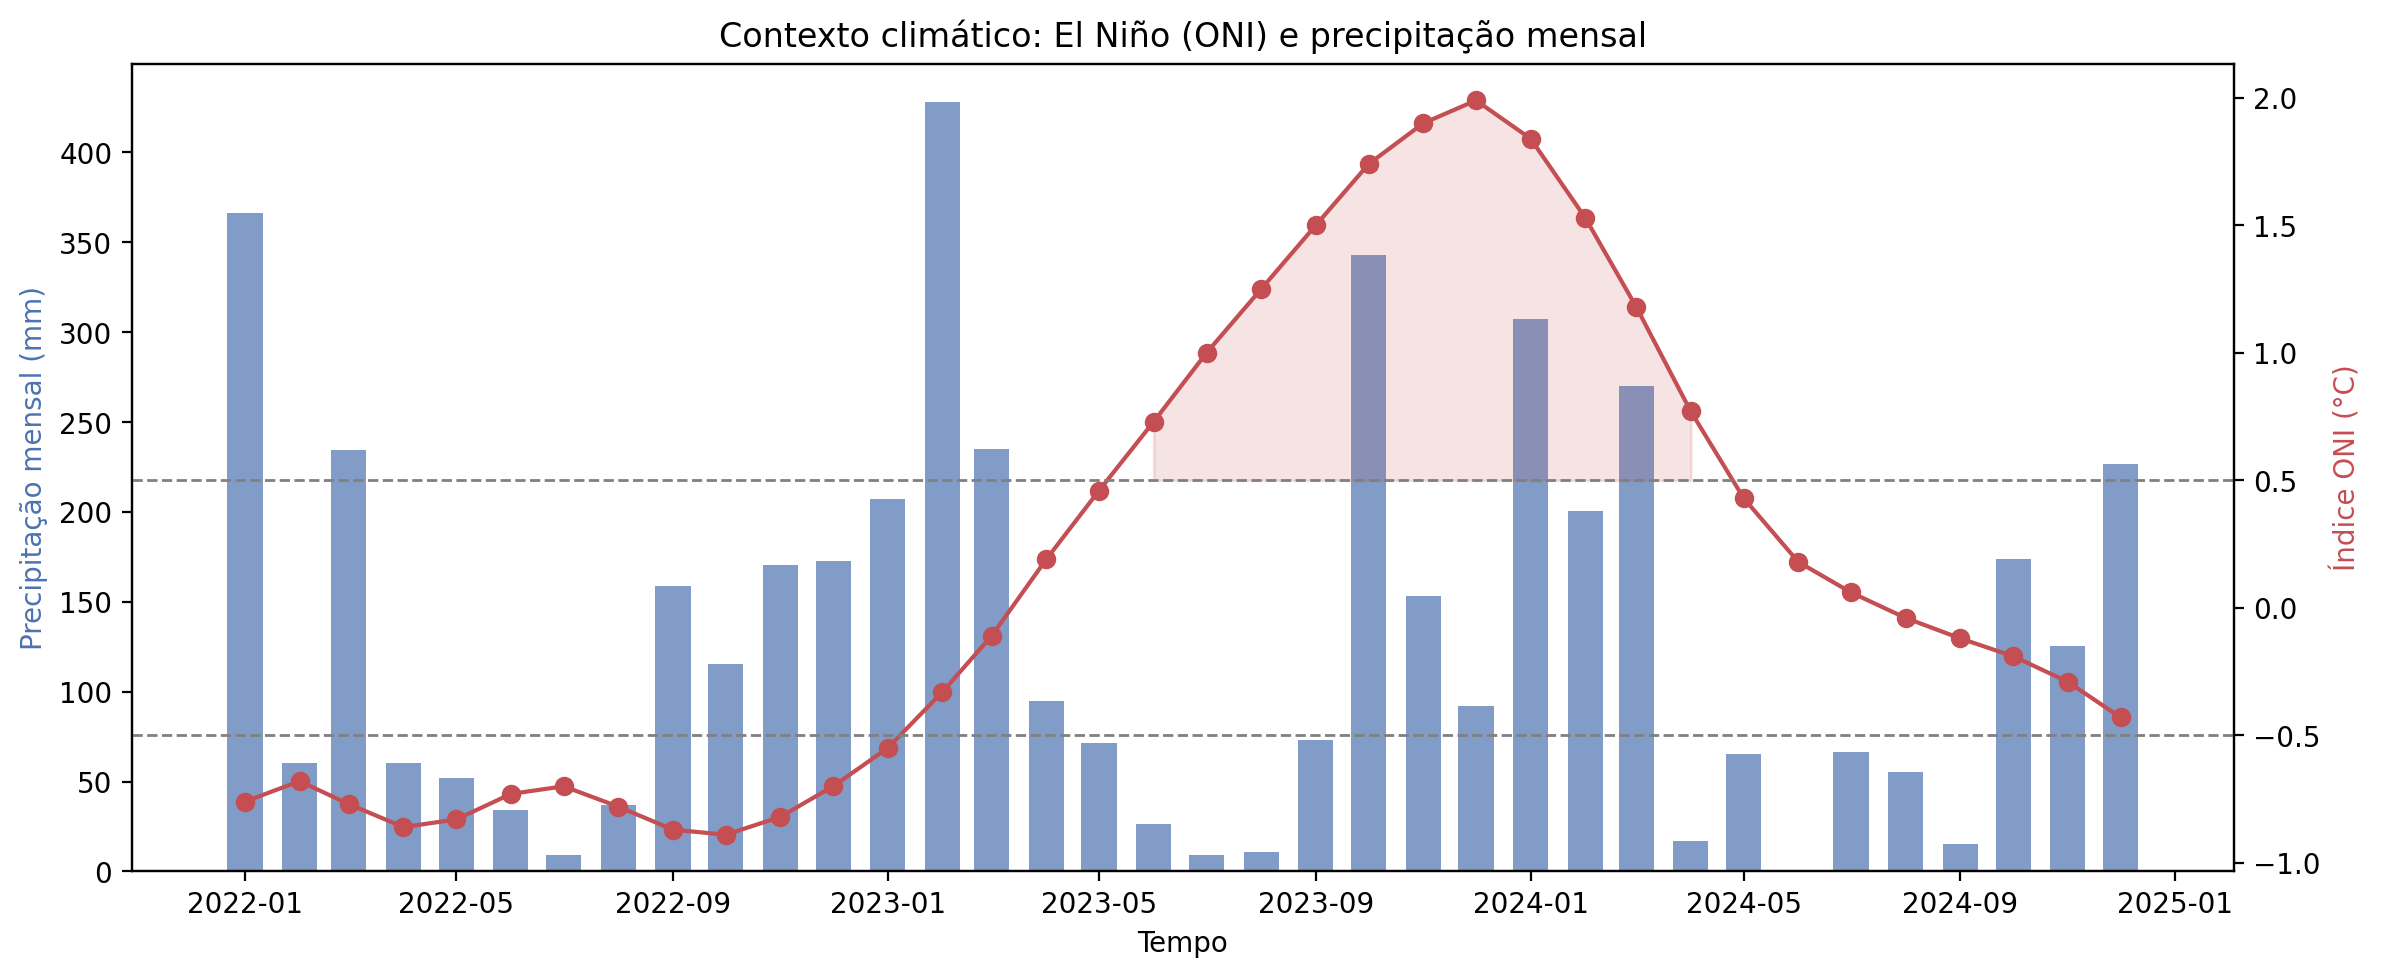
\includegraphics[width=\textwidth]{../figures/climate_context.png}
\caption{{\'I}ndice ONI (El Ni{\~n}o) e precipita{\c c}{\~a}o mensal da
esta{\c c}{\~a}o A701.}
\label{fig:climate}
\end{figure}

\begin{figure}[H]
\centering
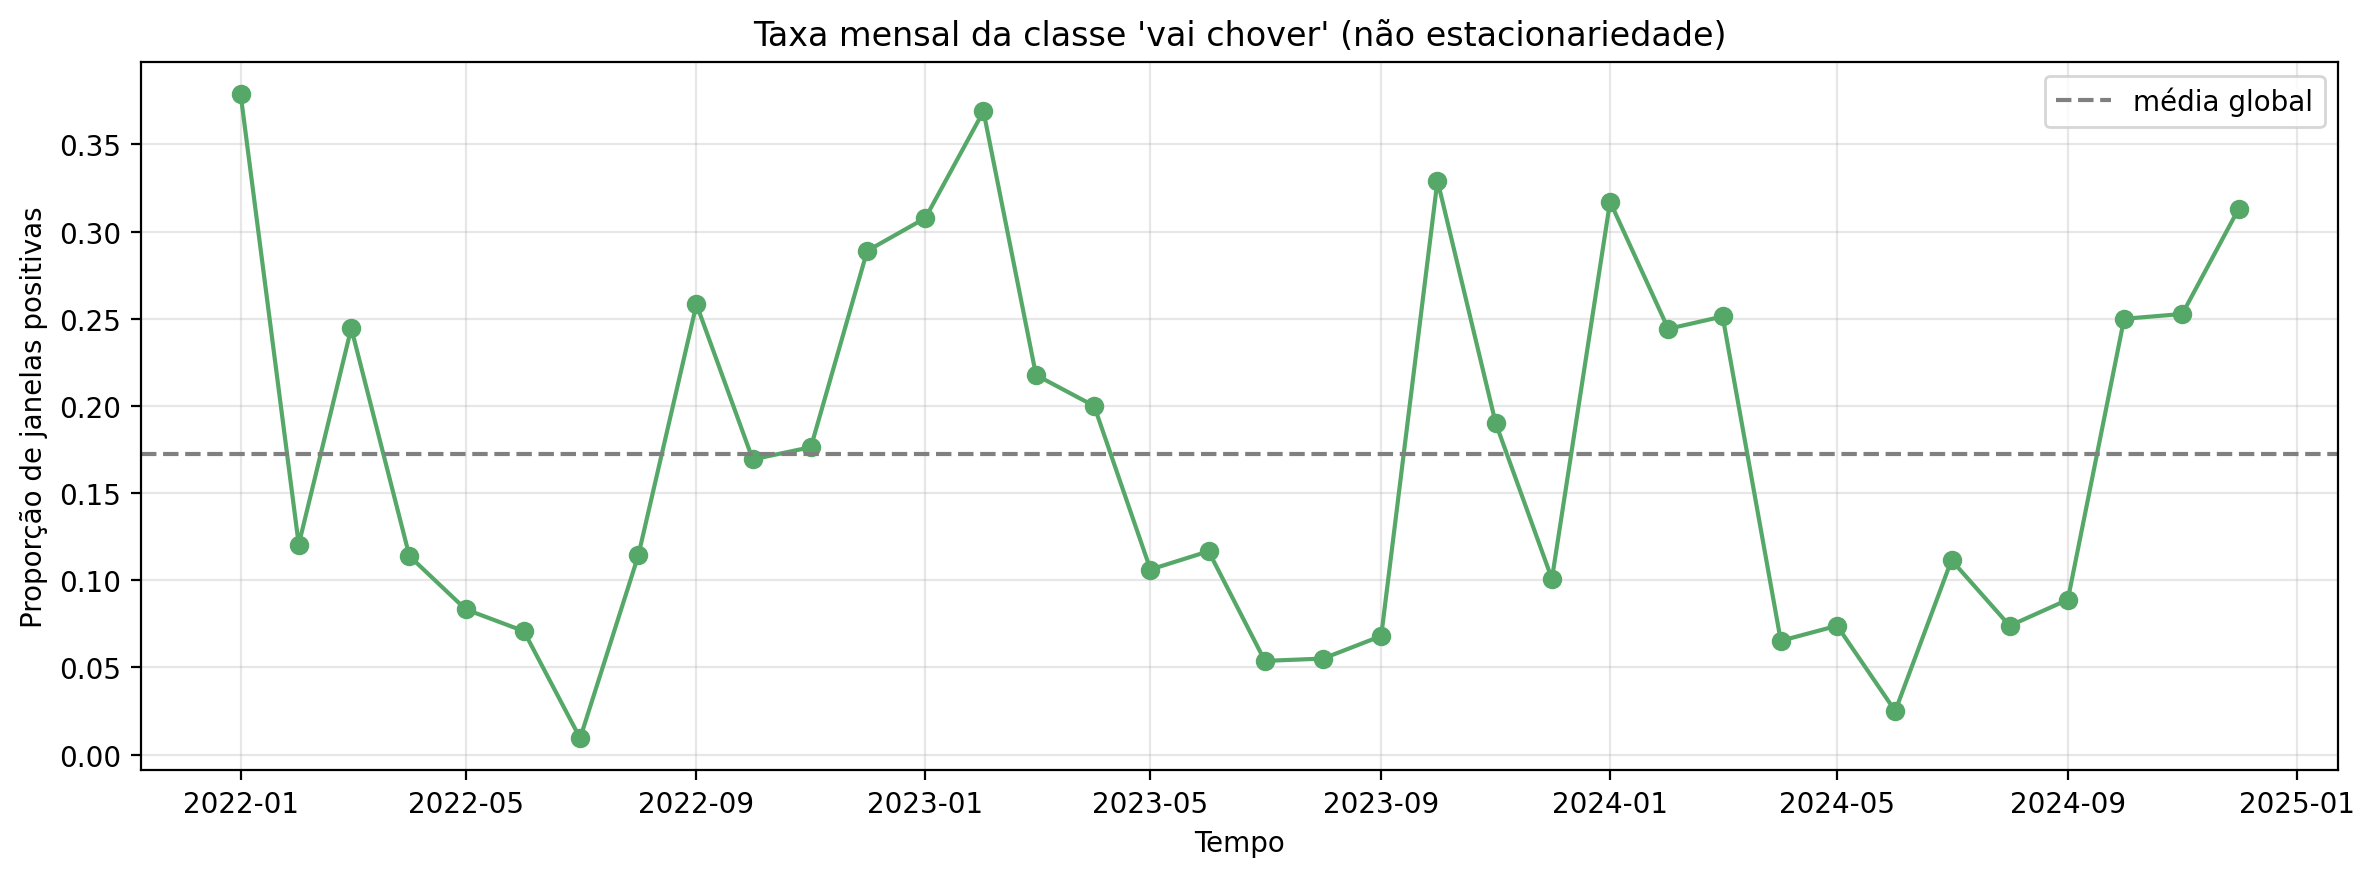
\includegraphics[width=\textwidth]{../figures/rain_nonstationarity.png}
\caption{Taxa mensal da classe ``vai chover'': a n{\~a}o estacionariedade
que torna o split cronol{\'o}gico mais dif{\'i}cil e mais honesto.}
\label{fig:nonstat}
\end{figure}

Essa n{\~a}o estacionariedade conecta o aspecto t{\'e}cnico ao social. Um
modelo avaliado por embaralhamento aleat{\'o}rio parece melhor porque
``revisita'' per{\'i}odos que j{\'a} conhece. No mundo real, por{\'e}m, a
previs{\~a}o {\'e} sempre sobre um futuro possivelmente diferente do passado --
e as mudan{\c c}as clim{\'a}ticas ampliam essa diferen{\c c}a, deslocando
regimes de chuva e intensificando extremos~\cite{rodrigues2024rs,
enso_subtropical2026}. Reportar apenas a m{\'e}trica aleat{\'o}ria, mais alta,
transmitiria falsa confian{\c c}a justamente nos cen{\'a}rios em que o alerta
{\'e} mais necess{\'a}rio.

\section{Conclusão}

O projeto implementou um classificador recorrente (LSTM/GRU) para prever chuva
de curto prazo a partir de janelas horárias de dados do INMET, enriquecidas
com o {\'i}ndice El Ni{\~n}o. A compara{\c c}{\~a}o controlada entre parti{\c
c}{\~a}o cronol{\'o}gica e aleat{\'o}ria quantificou o vazamento temporal: a
avalia{\c c}{\~a}o aleat{\'o}ria superestima o desempenho, e apenas a
parti{\c c}{\~a}o cronol{\'o}gica reflete o uso real. Al{\'e}m do resultado
num{\'e}rico, o estudo refor{\c c}a uma li{\c c}{\~a}o metodol{\'o}gica
essencial em aprendizado de m{\'a}quina aplicado ao clima: a forma de
particionar os dados pode ser mais decisiva para a validade das conclus{\~o}es
do que a escolha da arquitetura.

\bibliographystyle{plain}
\bibliography{references}

\end{document}
